\subsection{Revisions and Commits}

Both Revision in Subversion and Commit in Git are atomic changes fixed at certain moment in time by certain person with certain message. The translation of this metadata described below.

\subsubsection{From Revision to Commit}

This kind of translation depicted at diagram \ref{single_change_svn_to_git}.

\begin{figure}[!h]
\centering
\renewcommand{\figurename}{Diagram}
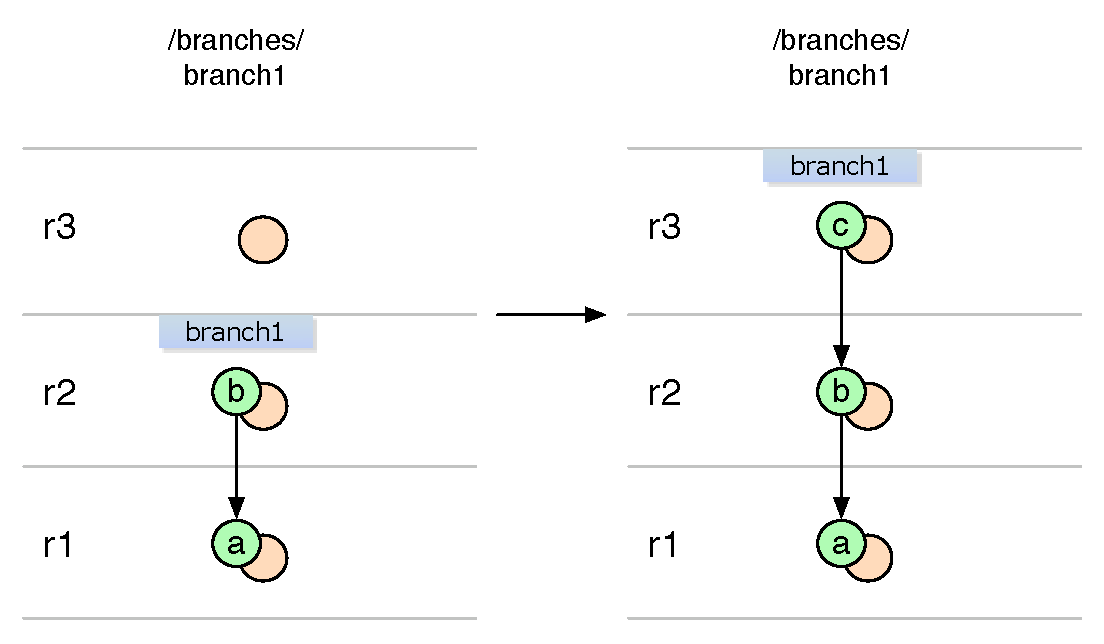
\includegraphics[width=\linewidth]{img/diagrams/single_change_svn_to_git.pdf}
\caption{Subversion revision being translated to Git commit.}
\label{single_change_svn_to_git}
\end{figure}

Subversion user modified /branches/branch1 at revision r3. For that change Translator
\begin{enumerate}
	\item Creates commit \emph{c} with Tree Object corresponding to /branches/branch1@r3 subdirectory content.
	\item Commit \emph{c} has Author Ident and Committer Ident corresponding to the author of the revision.
	\item Commit \emph{c} has the same date as revision r3.
	\item Commit \emph{c} has the same message as the revision r3.
	\item Commit \emph{c} has Parent Commit \emph{b} which corresponds to revision r2, i.e. previous modification of branch1.
	\item And finally Translator updates reference /refs/heads/branch2 to the created commit \emph{c}.
\end{enumerate}

\subsubsection{From Commit to Revision}

This kind of translation depicted at diagram \ref{single_change_git_to_svn}.

\begin{figure}[!h]
\centering
\renewcommand{\figurename}{Diagram}
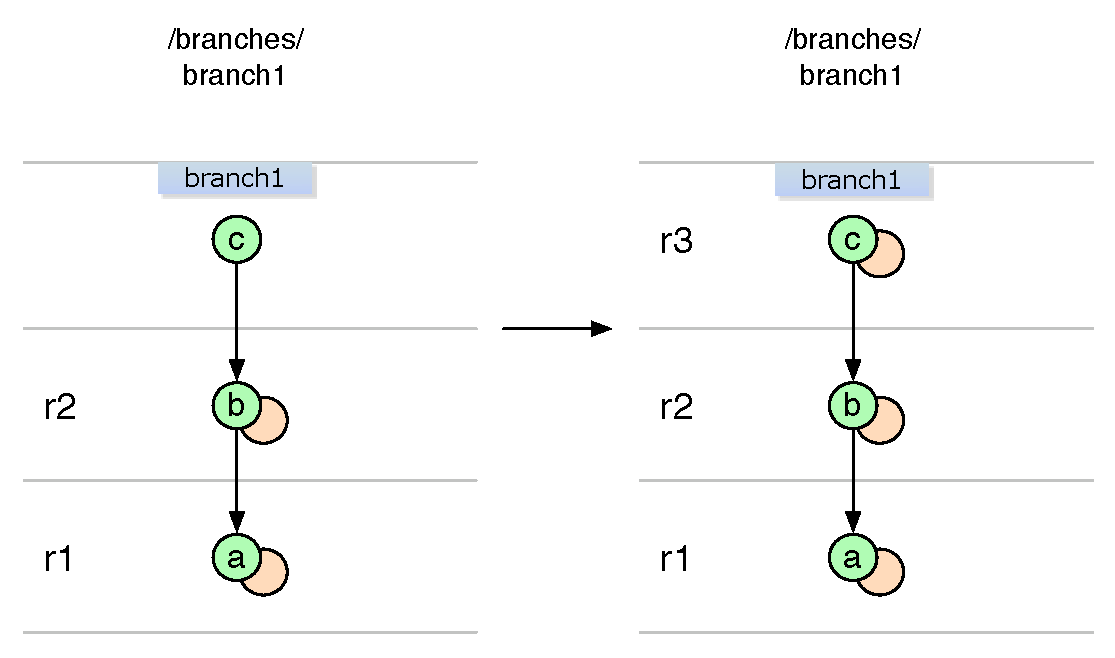
\includegraphics[width=\linewidth]{img/diagrams/single_change_git_to_svn.pdf}
\caption{Git commit being translated to Subversion revision.}
\label{single_change_git_to_svn}
\end{figure}

Git user created commit \emph{c} at \emph{branch1}. For that change Translator
\begin{enumerate}
	\item Creates revision \emph{r3}, /branches/branch1 subdirectory content corresponds to Tree Object of \emph{c} commit.
	\item Revision r3 \emph{c} has the author corresponding to author ident of commit \emph{c}.
	\item If the latest revision of Subversion repository before translation had date before commit \emph{c} creation date, this creation date is udsed for revision r3, otherwise the date of committing revision r3 is used.
	\item Revision r3 has the same message as commit \emph{c}.
\end{enumerate}

More complicated scenarios will be considered in the future chapters but metadata translation is common for any of them.